% this paper verifies the utility of loss functions previously not tested in OOD settings. We define sound-matching tasks with targets that cannot be matched by the synthesizer. This target sound is from a target synthesizer which has at least 1 critical parameter in common with the output synthesizer. The performance measure of interest here is how close can we approximate the difference in the set of critical parameters between the target and output synth. We call this proximity the partial parameter loss (PPL), and define it such that it can be taken as a reasonable measure of performance in each sound-matching test. 


For each sound-matching task, we use a bespoke  that measures the difference between the synthesizer parameters of interest. 

% \documentclass[runningheads,20pt]{llncs}


\documentclass[14pt]{extarticle} % also accepts 17pt, 20pt
\usepackage[top=0.5in,bottom=0.5in,left=0.5in,right=0.5in]{geometry}

\usepackage[T1]{fontenc}
\usepackage[utf8]{inputenc}
\usepackage{graphicx}
\usepackage{stfloats} % for positioning of figure* on the same page
\usepackage{caption}
\usepackage{tikz}
\usepackage[inline]{enumitem}
\usepackage[breaklinks=true,colorlinks=true, allcolors=blue]{hyperref}
\usepackage{breakcites}
\usepackage{microtype}
\usepackage{lipsum}
\usepackage{xcolor}
\usepackage{array}
\usepackage{float}
\usepackage{adjustbox}
\usepackage{listings}
\usepackage{csquotes}
\usepackage{makecell}
\usepackage{pdfpages}
\usepackage{xspace}
\usepackage{tikz}

\usetikzlibrary{positioning,shapes.geometric}

% to do:
% hearing tests
% one other way to present results is grouped by which losses are most appropriate for each situtation

\usepackage{xcolor}
\usepackage[utf8]{inputenc}       % For UTF-8 encoding
\usepackage{listings}
\usepackage{amsmath}              % Optional: for math symbols

\lstdefinelanguage{Faust}{
    morekeywords={import, process, environment, declare, with, if, else, while, for, int, float, true, false},
    sensitive=true,
    morecomment=[l]{//}, % Line comment
    morecomment=[s]{/*}{*/}, % Block comment
    morestring=[b]", % Strings
}

% Customize the appearance of the code
\lstset{
    language=Faust,
    backgroundcolor=\color{lightgray!20},
    basicstyle=\ttfamily\small,
    keywordstyle=\color{blue}\bfseries,
    stringstyle=\color{orange},
    commentstyle=\color{green}\itshape,
    showstringspaces=false,
    numbers=left,
    numberstyle=\tiny,
    frame=single,
    breaklines=true,
      basicstyle=\ttfamily,
  % literate={\delta}{{\(\delta\)}},
}


\captionsetup[lstlisting]{justification=centering, singlelinecheck=false}
\providecommand{\gls}[1]{#1}
\newcommand{\highlight}[1]{\textcolor[RGB]{00,150,00}{#1}}
\newcommand{\todo}[1]{\textcolor{red}{#1}}

\newcommand{\SIMSESpec}{\texttt{SIMSE\_Spec}\xspace}
\newcommand{\LoneSpec}{\texttt{L1\_Spec}\xspace}
\newcommand{\JTFS}{\texttt{JTFS}\xspace}
\newcommand{\DTWEnv}{\texttt{DTW\_Envelope}\xspace}
\newcommand{\OutDomain}{\textbf{Out-of-Domain Generation}\xspace}
\newcommand{\LossSelect}{\textbf{Loss Selection}}
\newcommand{\SynthSelect}{\textbf{Synthesis Selection}}
\newcommand{\PeriodicLoss}{\textbf{Periodic Loss}}

\newcommand{\BPNoise}{\textbf{BP-Noise}\xspace}
\newcommand{\BPSaw}{\textbf{BP-Saw}\xspace}
\newcommand{\AddSineSaw}{\textbf{Add-SineSaw}\xspace}
\newcommand{\AmpMod}{\textbf{Noise-AM}\xspace}
\newcommand{\FMMod}{\textbf{SineSaw-AM}\xspace}
\newcommand{\FMModvtwo}{\textbf{SineSine-AM}\xspace}
\newcommand{\PitchBendUp}{\textbf{PitchBend-Up}\xspace}

\begin{document}

\begin{abstract}
 Out-of-domain sound-matching is the task of automatically programming a synthesizer towards a sound that it cannot accurately replicate. Measuring performance in out-of-domain sound-matching is a difficult task to the subjective experience of sound, open-set recognition, characteristics of interest, etc. In addition, despite their critical role in sound-matching, the performance of different sound-similarity measures (or loss functions) under different circumstances has rarely been a topic of research. Should we be looking for a global sound-similarity measure, or is the choice of loss function a creative decision, much like the selection of a synthesizer?
 Here we present a series of differentiable out-of-domain sound-matching scenarios using four loss functions and various synthesizers. The experiments here are designed such that differences in parameters (whether all parameters or a subset) are well suited for measuring performance in sound-matching. The out-of-domain experiments here showcase the characteristics of the different loss functions, and confirm that their success is highly dependent on the method of synthesis and the target sound. 
\end{abstract}

\section{Introduction}
\label{sec:intro}
Manual sound design with a synthesizer is inherently iterative: an artist compares the synthesized output to a mental or auditory target, adjusts parameters, and repeats until the desired result is achieved~\cite{salimi2025soundmatching}.  
Differentiable iterative sound-matching automates this process by optimizing synthesizer parameters under the guidance of a loss function that measures similarity between a target and an output signal.  
Recent work has demonstrated that loss–synthesizer interactions are highly dependent on the synthesis method, with no universally optimal loss function across domains~\cite{salimi2025soundmatching}.  
That study established a systematic evaluation framework combining differentiable synthesizers, loss functions, and statistical ranking to reveal how different metrics succeed or fail depending on synthesis structure.

However, nearly all prior studies—including ours—assume an \emph{in-domain} setting, where the target and imitator synthesizers share identical architectures and parameterizations.  
This assumption simplifies evaluation but fails to represent real sound-design workflows.  
In practice, designers frequently attempt to imitate sounds created with other synthesizers, physical instruments, or recorded sources.  
Such settings define the \emph{out-of-domain} (OOD) sound-matching problem, where exact replication of the target signal is impossible and the goal shifts from \emph{parameter recovery} to \emph{perceptual imitation}.  
Despite its importance to creative audio practice, OOD sound-matching has received little systematic analysis and remains poorly understood.

In OOD conditions, only a subset of parameters can meaningfully correspond between the target and imitator.  
For instance, when matching a band-pass filtered saw wave with a noise synthesizer, the absolute pitch or harmonic content of the signal cannot align, yet the filter cutoffs can.  
To capture success in such scenarios, we introduce the \emph{partial parameter loss} (PPL), which measures the distance only over the critical subset of parameters expected to transfer perceptually between the target and imitator.  
PPL provides an interpretable performance measure for OOD experiments, enabling quantitative comparison even when large portions of the parameter space are unmatched or undefined.

Using the same differentiable iterative framework as in~\cite{salimi2025soundmatching}, we evaluate four loss functions—L1\_Spec, SIMSE\_Spec, DTW\_Envelope, and JTFS—across several controlled OOD scenarios designed to probe specific perceptual dimensions: (1) \textbf{band-pass filtering}, where cutoff frequencies are the critical features; (2) \textbf{amplitude modulation}, where modulation rates must align but carrier frequencies may not; and (3) \textbf{pitch-bending}, where temporal frequency trajectories differ by onset or curvature.  
For each scenario, we record 300 trials per loss function and analyze the resulting distributions of PPL values using bootstrapped ranking and the non-parametric Scott–Knott test.

\textbf{Objectives and Hypotheses.}  
This study extends differentiable iterative sound-matching into the OOD regime and tests the following hypotheses:
\begin{itemize}
  \item \textbf{H1:} Loss–synthesizer interactions observed in in-domain settings persist under OOD conditions, but with greater performance variability due to mismatched timbral attributes.
  \item \textbf{H2:} Context-sensitive losses such as DTW\_Envelope and SIMSE\_Spec yield higher PPL performance in OOD tasks where temporal or spectral envelopes are the dominant perceptual cues.
  \item \textbf{H3:} Agreement between automatic metrics and perceptual outcomes decreases under OOD conditions, emphasizing the need for feature-selective evaluation methods.
\end{itemize}
Together, these hypotheses aim to reveal whether loss functions can generalize beyond the boundaries of their training or design domain, and to identify which similarity measures best capture perceptual alignment when perfect reconstruction is unattainable.

\section{Background and Related Work}
\label{sec:background}

Sound-matching is the process of automatically programming a synthesizer to reproduce or imitate a target sound.  
Formally, it involves a parametric synthesizer $g(\theta)$, a target signal $x_0$, a representation function $\phi(\cdot)$, and a similarity measure $L(\theta, x_0) = d(\phi(g(\theta)), \phi(x_0))$, where $d$ denotes a distance metric.  
The objective is to find parameter settings $\theta^*$ that minimize $L$, yielding a synthesized output perceptually close to the target.  
This framework underlies both traditional and differentiable sound-matching approaches.

\subsection{In-Domain Sound-Matching}
Historically, sound-matching has been studied under \emph{in-domain} conditions, where the target and imitator synthesizers are identical.  
Early works relied on non-differentiable heuristics such as genetic algorithms and hill-climbers~\cite{horner1993machine,mitchell2007evolutionary}, which iteratively searched parameter spaces using spectral metrics.  
Subsequent approaches introduced supervised neural models that learned mappings between synthesizer parameters and audio outputs~\cite{yee2018automatic,esling2019flow,masuda2021soundmatch}. Such supervised approaches require access to large datasets of paired sounds and programs generated by the same synthesizer, limiting their applicability to cross-domain scenarios.

Recent research has revisited sound-matching through the lens of differentiable digital signal processing (DDSP)~\cite{engel2020ddsp}, where synthesizer modules and losses are implemented as differentiable operations.  
This has enabled gradient-based optimization of parameters directly through audio signals and feature representations.  
Within this framework, differentiable losses have included spectral losses based on short-time Fourier transforms (STFT or MSS), and more recent alternatives such as the joint time–frequency scattering (JTFS) transform~\cite{vahidi2023mesostructures} and differentiable dynamic-time-warping losses~\cite{salimi2025evaluating}.  
These measures have shown distinct strengths depending on synthesis method—e.g., spectrogram-based losses for subtractive synthesis and temporal-alignment losses for modulated tones—yet all were validated in in-domain contexts.

\subsection{Toward Out-of-Domain Sound-Matching}
The transition from in-domain to \emph{out-of-domain} (OOD) settings introduces a fundamental challenge: the target sound may not be realizable by the chosen synthesizer. OOD scenarios break the assumption of parameter correspondence, requiring the imitator to approximate perceptual rather than structural similarity, and therefore shift the goal from replication to imitation—seeking partial alignment on perceptually salient features such as amplitude envelopes or spectral balance.  
Despite its relevance, systematic OOD evaluation remains scarce~\todo{cite}

The evaluation of OOD success further complicates the problem.  
Metrics such as spectral L1 or mean-squared error are sensitive to global gain and timbral differences that may be irrelevant to perceived similarity.  
Even advanced feature-space losses like JTFS~\cite{vahidi2023mesostructures} have shown inconsistent behavior when temporal or spectral structures are mismatched~\cite{salimi2025soundmatching}.  
Few studies have attempted to isolate which aspects of the signal should be compared when full waveform alignment is unattainable.

\subsection{Gaps and Motivation}
We adopt a differentiable iterative framework similar to~\cite{salimi2025evaluating} but extend it to OOD scenarios where the target and imitator synthesizers differ in architecture or parameter range.  
We evaluate the ability of four differentiable loss functions—L1\_Spec, SIMSE\_Spec, DTW\_Envelope, and JTFS—to generalize under controlled cross-domain conditions.  
By introducing the partial parameter loss (PPL) as an evaluation metric, we aim to quantify how well each loss function preserves the critical transferable parameters of the target while tolerating unavoidable mismatches in other attributes.

This focus on controlled OOD experimentation and selective evaluation distinguishes the present work from prior DDSP studies and positions it as a step toward more generalizable, perceptually grounded sound-matching systems.


\section{Method Overview}
\label{sec:method_overview}

Our experimental design extends the differentiable iterative sound-matching framework introduced in~\cite{salimi2025evaluating} to controlled out-of-domain (OOD) scenarios.  
Each experiment pairs a target synthesizer $g_t$ and an imitator synthesizer $g$, which may differ in structure or parameterization, and optimizes $g$ for 200 gradient-based iterations under one of four differentiable loss functions: L1\_Spec, SIMSE\_Spec, JTFS, or DTW\_Envelope.  
Whereas in-domain matching seeks full parameter recovery, OOD matching emphasizes partial imitation of perceptually critical attributes that can meaningfully transfer across architectures.  

To quantify this partial success, we use the \textit{partial parameter loss} (PPL) as our performance metric.  
PPL measures distance only over the subset of parameters deemed critical for each scenario—for instance, filter cutoffs in band-pass matching or modulation rates in amplitude-modulated synthesis—while ignoring parameters without interpretable correspondence, such as oscillator pitch or waveform shape.  
For each combination of $(g_t, g, L)$, 300 trials are conducted to produce a distribution of PPL values.  
The distributions are bootstrapped to 1000 samples and compared using the non-parametric Scott–Knott (\gls{NPSK}) test to obtain ranked performance across loss functions.  

This design enables a systematic investigation of how different differentiable similarity measures generalize beyond their native synthesis domain, and whether their relative strengths—observed previously under in-domain conditions—remain consistent when perfect reproduction of the target is impossible.

 \section{Methodology}
\label{sec:experiment_setup}

\subsection{Experimental Framework}
The iterative optimization loop shown in Fig.~\ref{fig:sound_design_loop_iterative} forms the foundation of all experiments.  
In each trial, a target synthesizer $g_t$ is selected, and a target sound $x = g_t(\theta_t)$ is generated using randomly sampled parameters $\theta_t$.  
An imitator synthesizer $g$ and a loss function $L$ are then chosen, and $g$ is optimized for 200 gradient-based iterations.  
Unless otherwise specified, $g \neq g_t$, corresponding to an out-of-domain (OOD) configuration.

Each \textbf{trial} consists of a single 200-iteration optimization run, resulting in one final \textit{partial parameter loss} (PPL) value.  
An \textbf{experiment} comprises 300 independent trials with the same $(L, g, g_t)$ configuration, yielding a distribution of 300 PPL values.  
A \textbf{scenario} consists of four such experiments—one per loss function—using the same synthesizer pair $(g_t, g)$.  
Comparing the four distributions reveals which loss function best supports imitation for that particular scenario.

The 300 PPL values from each experiment are upsampled by bootstrapping to 1000 samples of the mean, each drawn with replacement from the full distribution~\cite{tibshirani1993introduction,chernick2011bootstrap}.  
The resulting bootstrapped distributions are compared using the non-parametric Scott–Knott (\gls{NPSK}) test~\cite{tantithamthavorn2017mvt,tantithamthavorn2018optimization}, which partitions loss functions into statistically distinct ranks.  
Ranks range from~1 (best-performing) to~4 (worst-performing), with the possibility of ties when distributions are not significantly different.

\subsection{Partial Parameter Loss (PPL)}
In out-of-domain sound-matching, many parameters of the target and imitator synthesizers do not correspond directly—for example, when the target employs a saw oscillator but the imitator uses noise, or when modulation structures differ.  
To evaluate only the aspects of the signal that can meaningfully transfer across domains, we compute a \emph{partial parameter loss} (PPL).  

PPL measures the L1 distance only across the subset of parameters considered perceptually critical for the scenario:
\begin{equation}
\mathrm{PPL} = \| \theta^{(\mathrm{crit})}_t - \hat{\theta}^{(\mathrm{crit})} \|_1,
\end{equation}
where $\theta^{(\mathrm{crit})}$ denotes the target’s critical parameters (e.g., filter cutoffs, modulation rates) and $\hat{\theta}^{(\mathrm{crit})}$ the corresponding recovered parameters of the imitator.  
Parameters with no perceptual or structural correspondence (e.g., oscillator frequency, waveform type) are ignored.  
This enables a fair and interpretable comparison across mismatched synthesizers.

\subsection{Scenario 1: Band-Pass Matching}
The first scenario investigates band-pass filtering in noise and saw-wave synthesizers.  
The target synthesizer $g_t$ is \BPSaw (Listing~\ref{lst:program0_saw}), and the imitator $g$ is \BPNoise (Listing~\ref{lst:program0}).  
The task is defined as reproducing the high-pass and low-pass cutoff frequencies of the target’s band-pass filter, ignoring differences in excitation signal (noise vs. saw).

Since filter cutoffs are directly reflected in the spectral envelope, spectrogram-based loss functions are expected to perform best.  
Indeed, the results in Fig.~\ref{fig:npsk_BP} show that \SIMSESpec\ consistently achieves the lowest PPL, confirming its robustness to amplitude scaling and its suitability for filter-based imitation tasks.

\begin{lstlisting}[caption={\BPNoise}, label={lst:program0}, language=Faust,
float, floatplacement=!H, xleftmargin=1em, xrightmargin=0.5em, firstnumber=0, aboveskip=0em, belowskip=-1em]
import("stdfaust.lib");
lp_cut = hslider("lp_cut",900,100,5000,5);
hp_cut = hslider("hp_cut",100,1,400,5);
process = no.noise:fi.lowpass(3,lp_cut):fi.highpass(10,hp_cut);
\end{lstlisting}

\begin{lstlisting}[caption={\BPSaw}, label={lst:program0_saw}, language=Faust,
float, floatplacement=!H, xleftmargin=1em, xrightmargin=0.5em, firstnumber=0, aboveskip=0em, belowskip=-1em]
import("stdfaust.lib");
lp_cut = hslider("lp_cut", 2801, 100, 5000, 1);
hp_cut = hslider("hp_cut", 142, 1, 400, 1);
sawOsc(f) = +(f/ma.SR) ~ ma.frac;
process = sawOsc(30):fi.lowpass(5, lp_cut):fi.highpass(5, hp_cut);
\end{lstlisting}

\begin{figure}[htbp]
  \centering
  \scriptsize
  \begin{minipage}{\columnwidth}
    \begin{minipage}{0.10\columnwidth}
      \raggedleft
      \vspace{0.5cm}
      SIMSE\\[0.6cm]
      L1\\[0.65cm]
      JTFS\\[0.65cm]
      DTW
    \end{minipage}%
    \begin{minipage}{0.88\columnwidth}
      \centering
      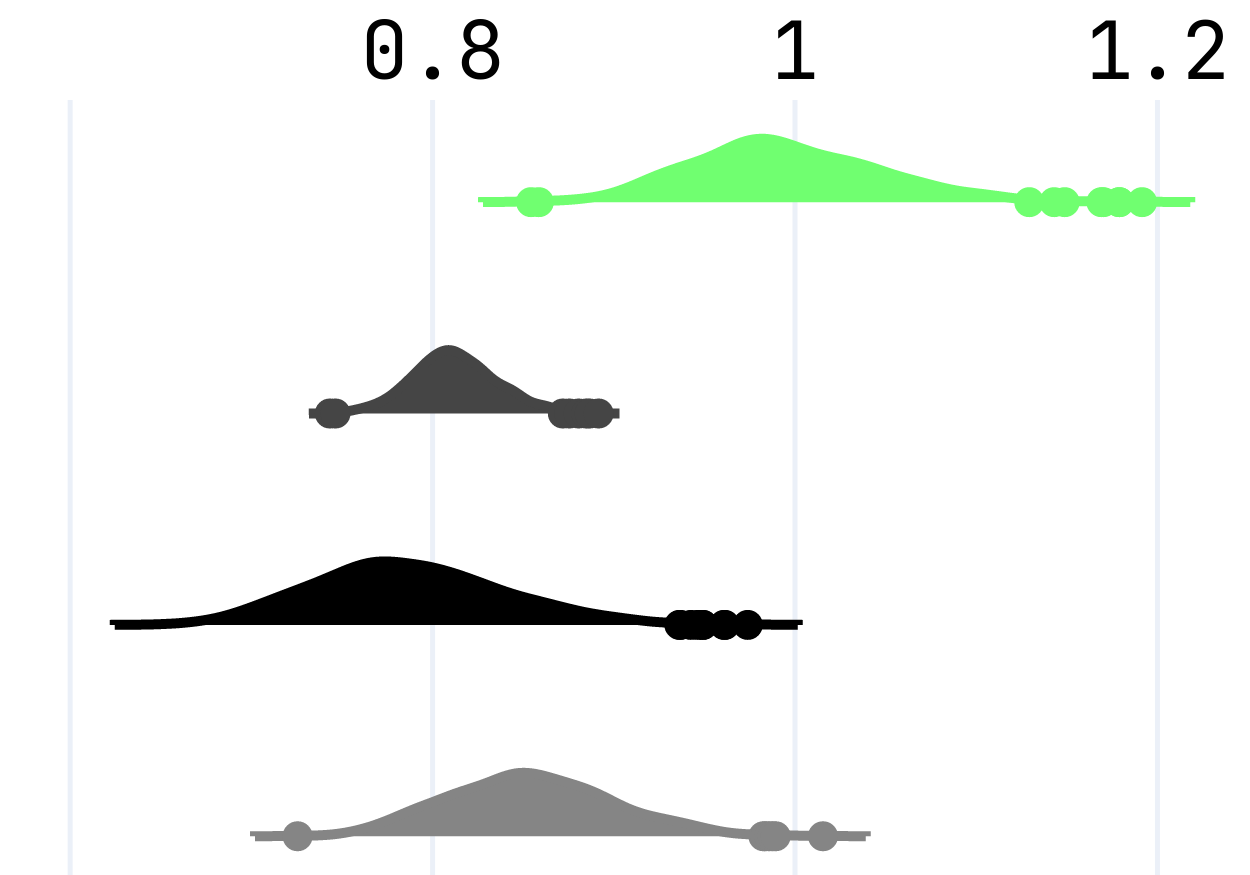
\includegraphics[width=\linewidth]{images/npsk_ood_P_Loss_3.png}
    \end{minipage}
  \end{minipage}
  \caption{Bootstrapped distributions and NPSK ranks for band-pass sound matching.}
  \label{fig:npsk_BP}
\end{figure}

\subsection{Scenario 2: AM Synthesizer Matching}
Amplitude-modulated synthesizers are ideal for evaluating temporal envelope sensitivity, as carrier frequencies and harmonic structures differ significantly across domains.  
We test three variants using the synthesizers \FMMod\ (Listing~\ref{lst:program3}) and \FMModvtwo\ (Listing~\ref{lst:program3_v2}).  
\FMMod\ modulates a saw oscillator’s amplitude with a sinusoidal LFO, while \FMModvtwo\ uses sine oscillators for both carrier and modulator.  
In all cases, the \texttt{amp} parameter (LFO frequency) defines the rate of amplitude modulation and is treated as the critical component for PPL evaluation; the \texttt{car} parameter (carrier frequency) is ignored, as it cannot align across domains.

\begin{lstlisting}[caption={\FMMod}, label={lst:program3},language=Faust,float,floatplacement=!H,xleftmargin=1em,xrightmargin=0.5em,firstnumber=0,aboveskip=0em, belowskip=-1em]
import("stdfaust.lib");
carrier = hslider("car",car_a,car_b,car_c,1);
amp = hslider("amp",amp_a,amp_b,amp_c,1);
sineOsc(f) = +(f/ma.SR) ~ ma.frac:*(2*ma.PI) : sin;
sawOsc(f) = +(f/ma.SR) ~ ma.frac;
process = sineOsc(amp)*sawOsc(car);
\end{lstlisting}

\begin{lstlisting}[caption={\FMModvtwo}, label={lst:program3_v2},language=Faust,float,floatplacement=!H,xleftmargin=1em,xrightmargin=0.5em,firstnumber=0,aboveskip=0em, belowskip=-1em]
import("stdfaust.lib");
carrier = hslider("car",car_a,car_b,car_c,1);
amp = hslider("amp",amp_a,amp_b,amp_c,1);
sineOsc(f) = +(f/ma.SR) ~ ma.frac:*(2*ma.PI) : sin;
process = sineOsc(amp)*sineOsc(car);
\end{lstlisting}

Three OOD conditions are tested:
\begin{enumerate}
  \item \textbf{Non-overlapping carrier frequencies}: target and imitator carriers occupy disjoint frequency ranges (30–250~Hz vs.~1000–5000~Hz).  
  \item \textbf{Sine target, saw imitator}: \FMModvtwo\ as target and \FMMod\ as imitator.  
  \item \textbf{Saw target, sine imitator}: the reverse of condition~2.  
\end{enumerate}

Across all conditions, the DTW\_Envelope loss function performs best (see Fig.~\ref{fig:npsk_am_synths}), reflecting its ability to capture envelope-based temporal similarity despite mismatched spectral structures.

\begin{figure*}[t]
  \centering
  \begin{minipage}[t]{\textwidth}
    % Left-side labels
    \begin{minipage}[t]{0.045\textwidth}
      \footnotesize\raggedleft
      \vspace{-2.75cm} % align with top of images
      SIMSE\\[0.4cm]
      L1\\[0.385cm]
      JTFS\\[0.365cm]
      DTW
    \end{minipage}%
    \hspace{0.01\textwidth}%
    % Right side: images + captions
    \begin{minipage}[t]{0.91\textwidth}
      \centering
      \begin{minipage}[t]{0.31\textwidth}
        \centering
        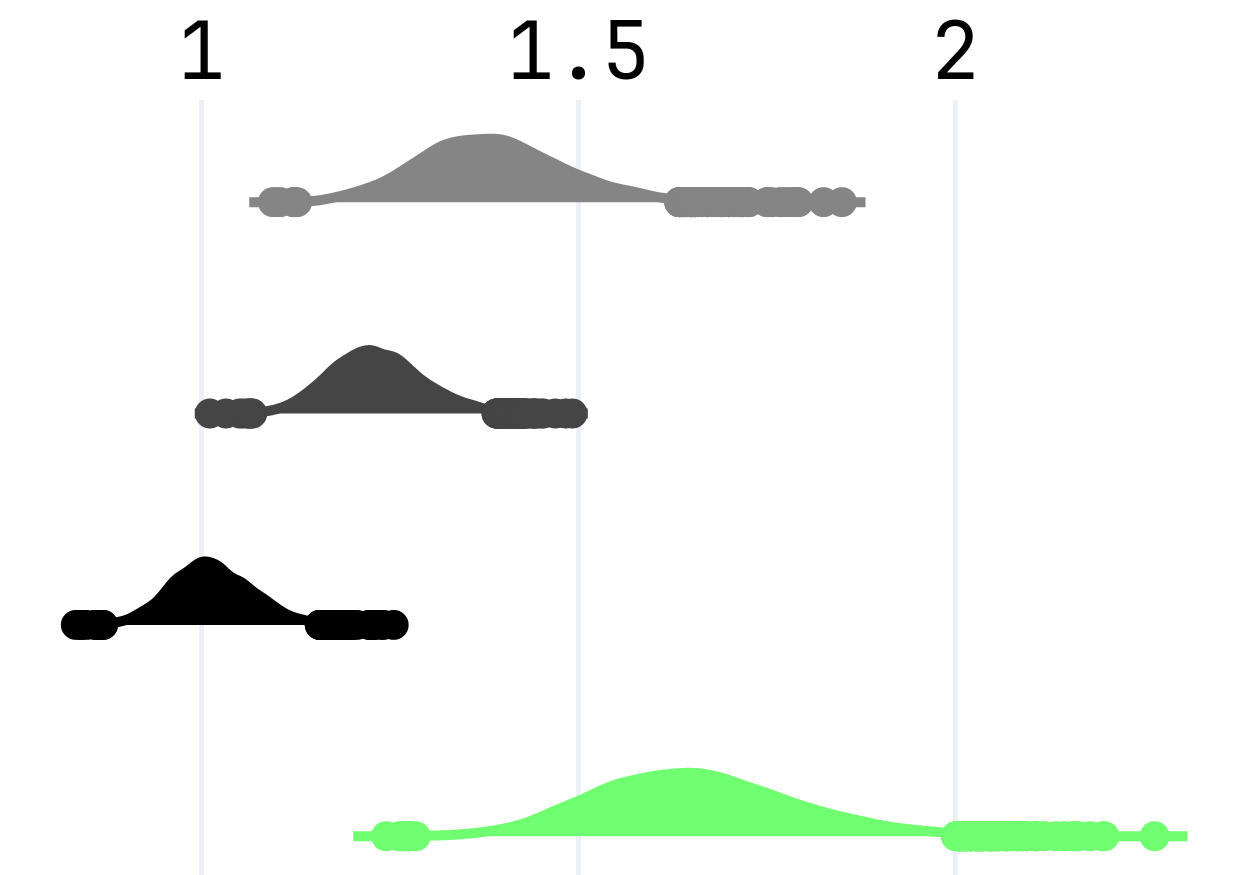
\includegraphics[width=\linewidth]{images/npsk_ood_P_Loss_0.png}
        \vspace{0.3em}
        \footnotesize (a)~Non-Overlapping Frequencies
      \end{minipage}
      \hspace{0.015\textwidth}%
      \begin{minipage}[t]{0.31\textwidth}
        \centering
        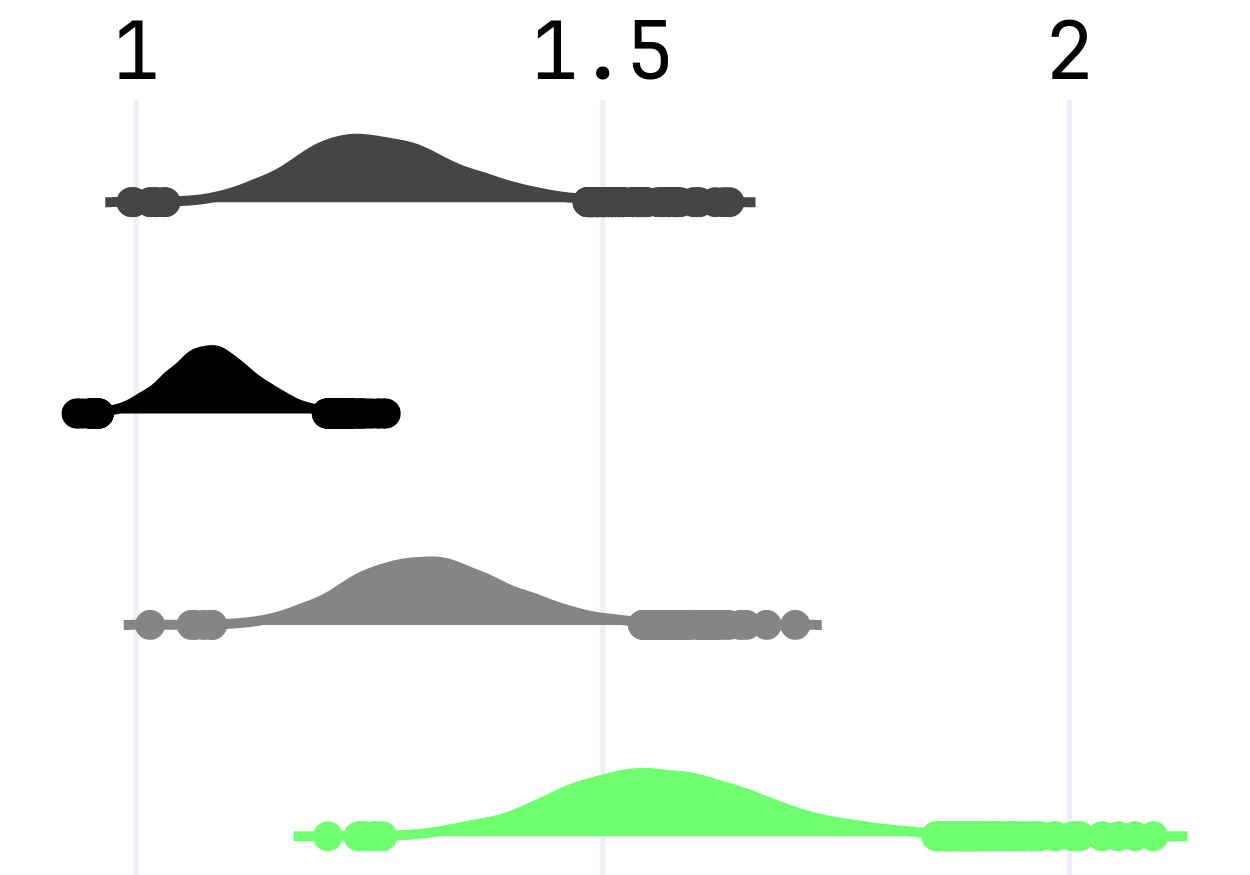
\includegraphics[width=\linewidth]{images/npsk_ood_P_Loss_1.png}
        \vspace{0.3em}
        \footnotesize (b)~Sine Target, Saw Imitator
      \end{minipage}
      \hspace{0.015\textwidth}%
      \begin{minipage}[t]{0.31\textwidth}
        \centering
        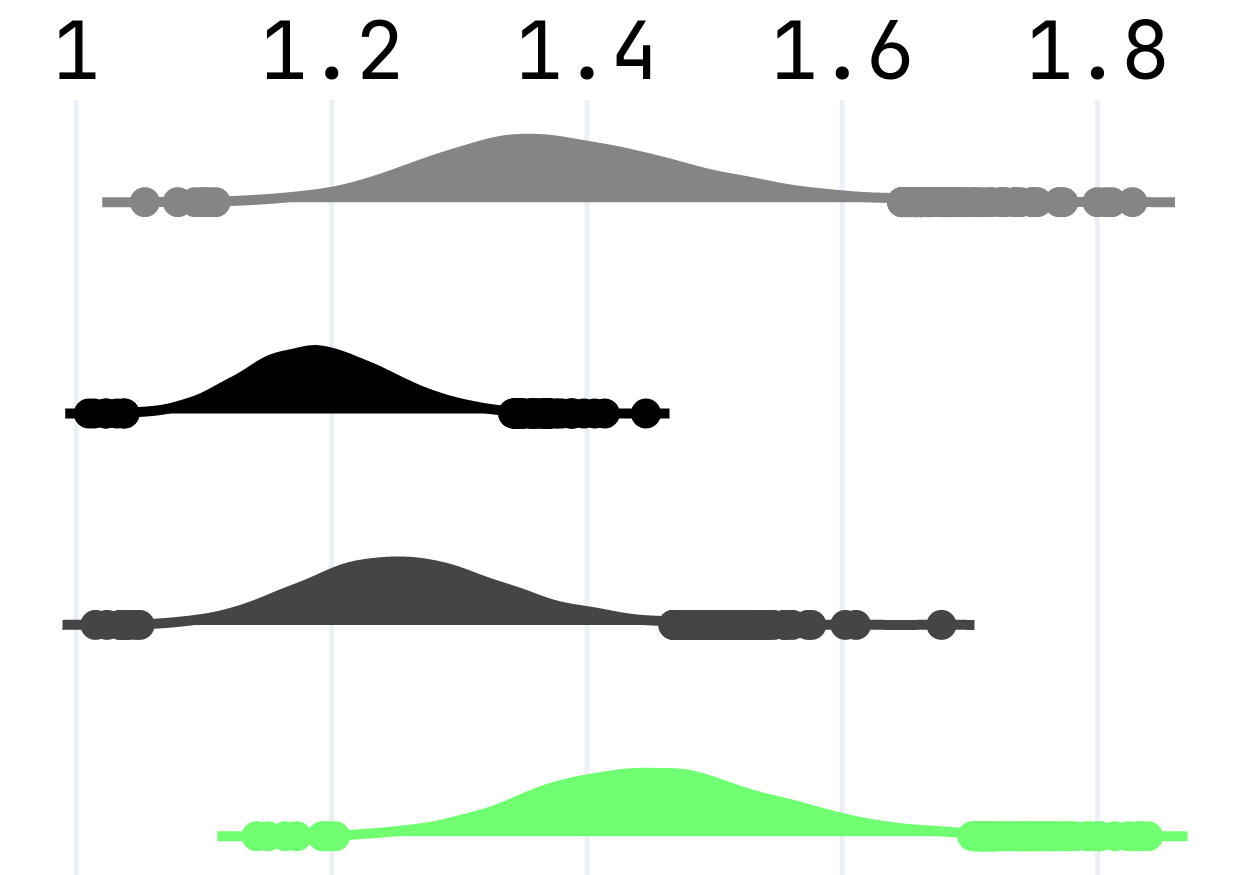
\includegraphics[width=\linewidth]{images/npsk_ood_P_Loss_2.png}
        \vspace{0.3em}
        \footnotesize (c)~Saw Target, Sine Imitator
      \end{minipage}
    \end{minipage}
  \end{minipage}
  \caption{Bootstrapped distributions and ranks for AM-Synthesizer sound matching.}
  \label{fig:npsk_am_synths}
\end{figure*}


\subsection{Scenario 3: Pitch-Bending}
The final set of experiments examines pitch-bending synthesizers, adapted from chirplet-style models used in~\cite{vahidi2023mesostructures}.  
Here, the target and imitator differ by a temporal offset, curvature, or modulation pattern in the pitch trajectory, creating various degrees of OOD mismatch.  
The search parameters include the starting pitch (30–500~Hz) and the exponential rate of pitch increase (1–20 samples per step).  
Three variations are evaluated:
\begin{enumerate}
  \item \textbf{Delayed pitch-bending}: imitator must match a target with a random delay before the bend onset.  
  \item \textbf{No-delay pitch-bending}: same synthesizer pair but without delay (in-domain control).  
  \item \textbf{Pulsating pitch-bending}: adds a periodic modulation on top of the exponential bend to test mesostructural sensitivity.
\end{enumerate}

As shown in Fig.~\ref{fig:npsk_pitch_bends}, \JTFS\ performs well when timing alignment is preserved (scenario~2), but its advantage diminishes when local temporal offsets or composite modulations are introduced.  
DTW\_Envelope outperforms others under delayed and pulsating conditions, confirming its strength in capturing envelope-level temporal similarity.

\begin{figure*}[t]
  \centering
  % Left-side labels
  \begin{minipage}[t]{0.045\textwidth}
    \footnotesize\raggedleft
    \vspace{-3cm} % align with top of images
    SIMSE\\[0.4cm]
    L1\\[0.385cm]
    JTFS\\[0.365cm]
    DTW
  \end{minipage}%
  \hspace{0.01\textwidth}%
  % Right-side: reordered minipage images
  \begin{minipage}[t]{0.94\textwidth}
    \centering
    \begin{minipage}[t]{0.31\textwidth}
      \centering
      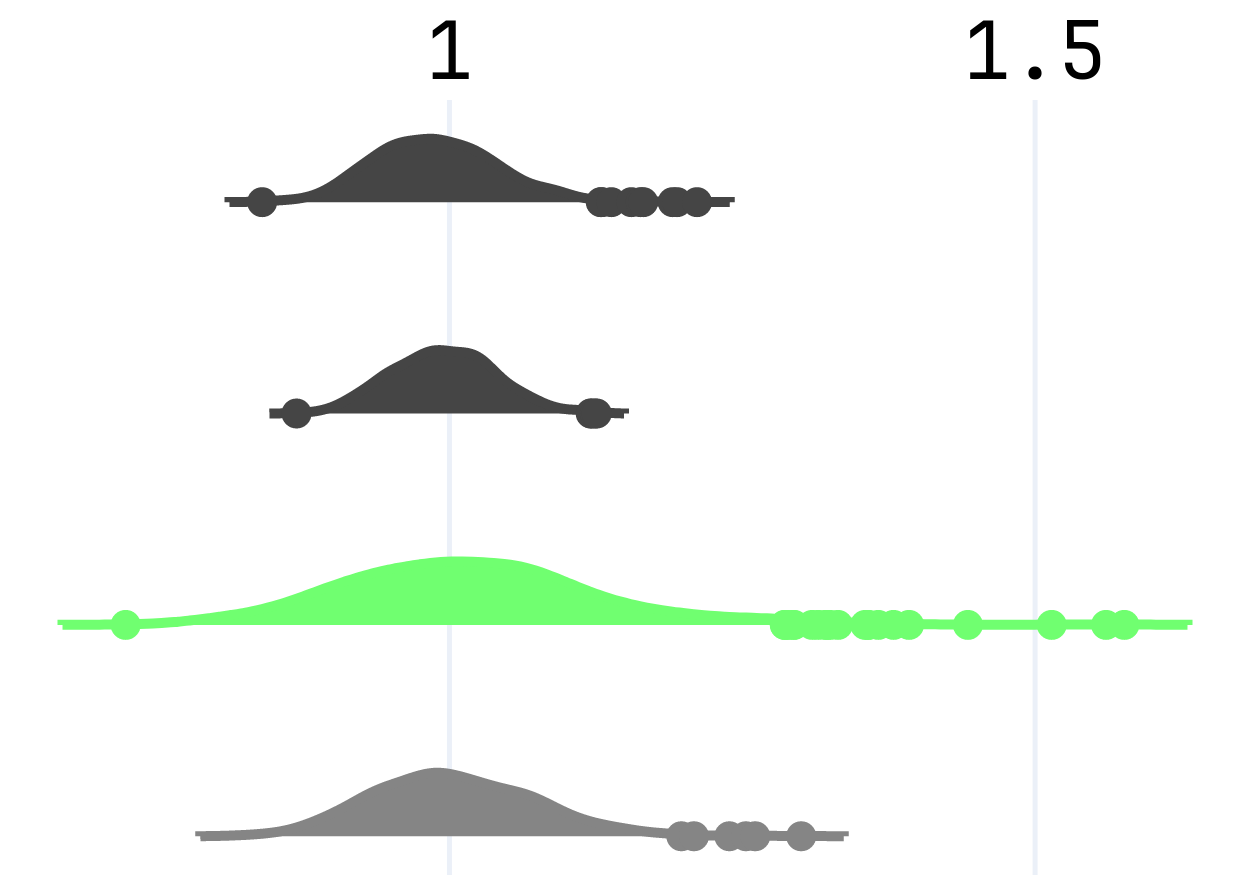
\includegraphics[width=\linewidth]{images/npsk_ood_P_Loss_6.png}
      \vspace{0.3em}
      \footnotesize (a)~Delayed Pitch-bend
    \end{minipage}
    \hspace{0.015\textwidth}
    \begin{minipage}[t]{0.31\textwidth}
      \centering
      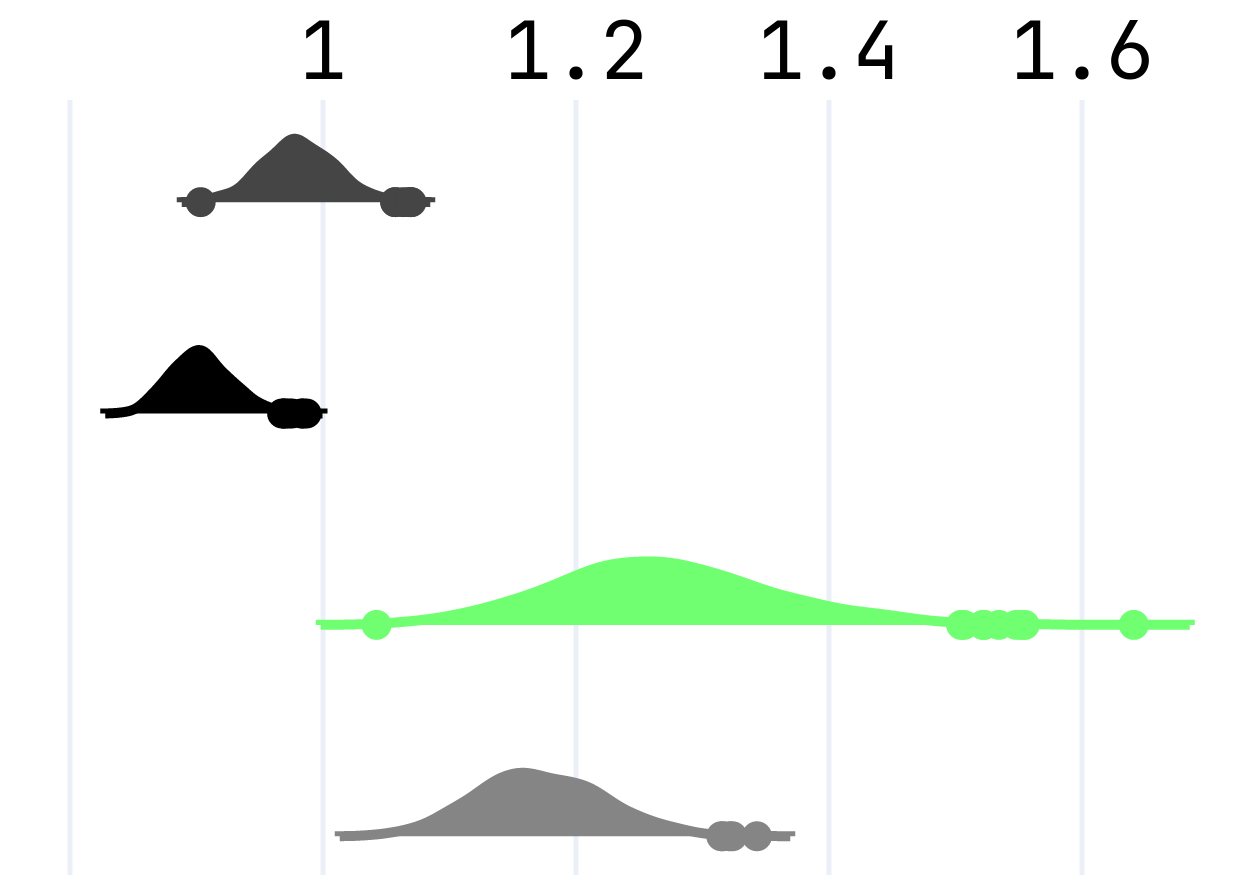
\includegraphics[width=\linewidth]{images/npsk_ood_P_Loss_4.png}
      \vspace{0.3em}
      \footnotesize (b)~No-delay Pitch-bend
    \end{minipage}
    \hspace{0.015\textwidth}
    \begin{minipage}[t]{0.31\textwidth}
      \centering
      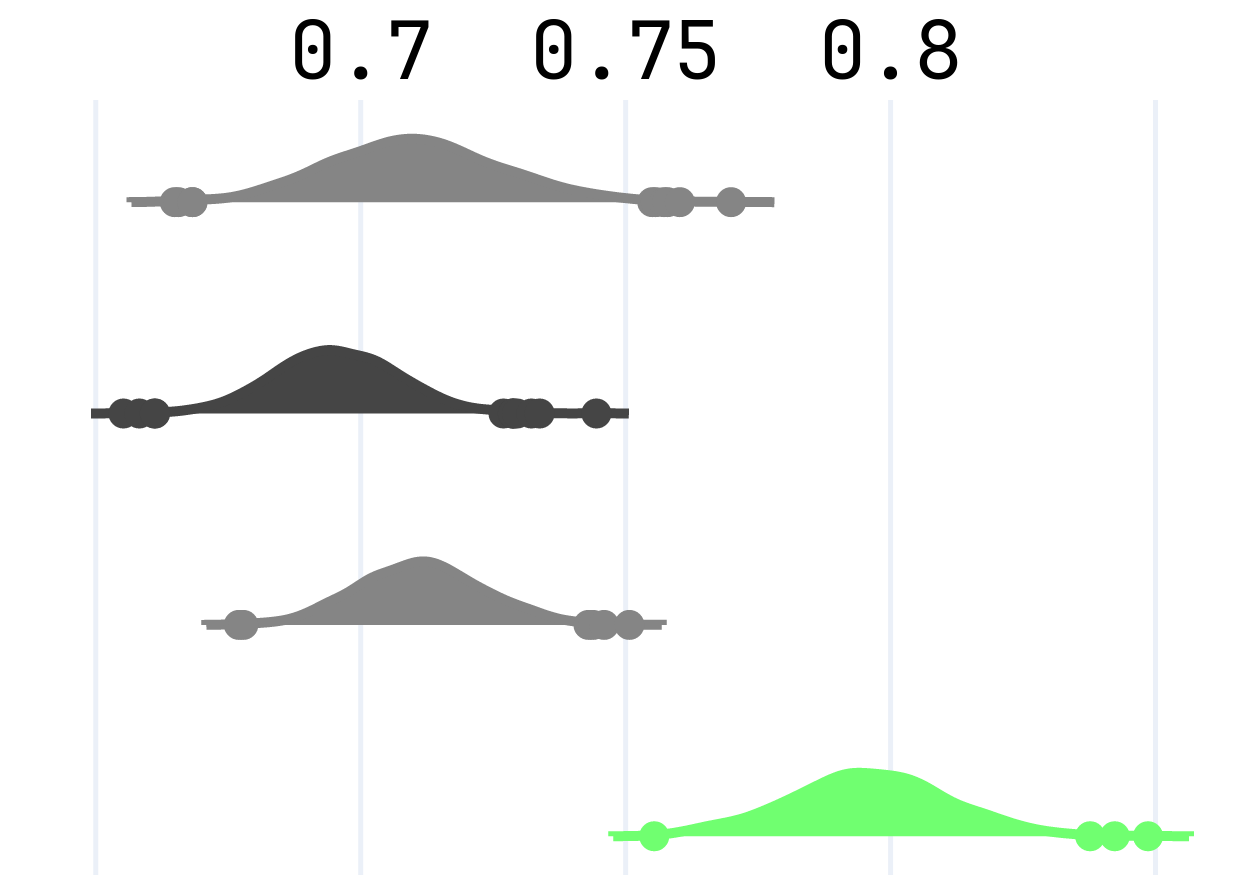
\includegraphics[width=\linewidth]{images/npsk_ood_P_Loss_5.png}
      \vspace{0.3em}
      \footnotesize (c)~Pulsating Pitch-bend
    \end{minipage}
  \end{minipage}
  \caption{Bootstrapped distributions and ranks for non-delayed, randomly delayed, and pulsating pitch-bend programs.}
  \label{fig:npsk_pitch_bends}
\end{figure*}



\bibliographystyle{alpha}
\bibliography{references}

\end{document}


